\subsection{Tasking Extensions}
\label{sub:tasking}

%% BRONIS: We should  cover 4.0 and 4.5 tasking extensions
%% BRONIS: Specifically: Discuss task dependences, taskgroup and taskloop

%% STEPHEN: Introduce the problem with OpenMP 3.x

Directives to support asynchronous task parallelism were first introduced in OpenMP 3.0, and the initial design rationale for this capability is explained in an article by Ayguad\'{e} et al.~\cite{ayguade2009tpds}.  Along with task generation using the \texttt{task} construct, task synchronization is provided using the \texttt{taskwait} construct and barriers.  The \texttt{taskwait} construct specifies a wait on the completion of child tasks of the current task, and a barrier requires complete execution of all tasks in the current parallel region before any threads in the team are allowed to continue execution beyond the barrier.  In many instances, these simple synchronization mechanisms lack the expressiveness to fully expose all available application parallelism.  OpenMP 4 addresses such limitations with two additional synchronization mechanisms, task dependences and task groups.


%% SMATEO: this is a bit ugly, but it's the only way I know to do it :D
\begin{figure}

\newsavebox{\firstExample}
\newsavebox{\secondExample}

\begin{lrbox}{\firstExample}
%\begin{minipage}{0.48\columnwidth}
\begin{minipage}{0.45\columnwidth}
%\begin{minted}[fontsize=\small]{c}
\begin{minted}{c}
#pragma omp task
produce(a);
#pragma omp task
produce(b);
#pragma omp task
produce(c);

// wait on all
//    three child
//    tasks here
#pragma omp \
        taskwait

#pragma omp task
consume(a, b);
#pragma omp task
consume(b, c);
#pragma omp task
consume(a, c);
\end{minted}
\end{minipage}
\end{lrbox}

\begin{lrbox}{\secondExample}
%\begin{minipage}{0.48\columnwidth}
\begin{minipage}{0.50\columnwidth}
%\begin{minted}[fontsize=\small]{c}
\begin{minted}{c}
#pragma omp task \
    depend(out: a)
produce(a);
#pragma omp task \
    depend(out: b)
produce(b);
#pragma omp task \
    depend(out: c)
produce(c);

#pragma omp task \
   depend(in: a, b)
consume(a, b);
#pragma omp task \
   depend(in: b, c)
consume(b, c);
#pragma omp task \
   depend(in: a, c)
consume(a, c);
\end{minted}
\end{minipage}
\end{lrbox}



\subfloat[][OpenMP 3.0]{\usebox{\firstExample}\label{fig:CodeTaskDeps3.0code}}
~
~
\subfloat[][OpenMP 4.0]{\usebox{\secondExample}\label{fig:CodeTaskDeps4.0code}}

\centering{\subfloat{
\includegraphics[width=0.30\columnwidth]{pics/intro_tasking_ex1_legend.png}}}
\addtocounter{subfigure}{-1}

\subfloat[][]{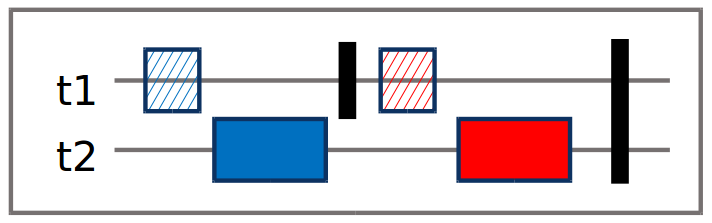
\includegraphics[width=0.48\columnwidth]{pics/intro_tasking_ex1_omp3.png}\label{fig:CodeTaskDeps3.0timeline}}
~
~
\subfloat[][]{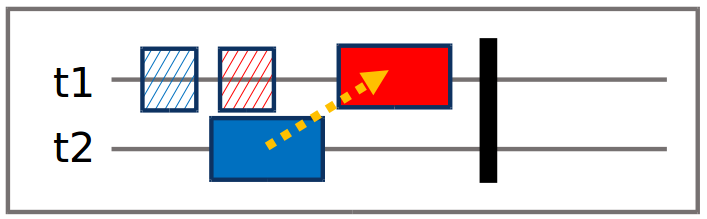
\includegraphics[width=0.48\columnwidth]{pics/intro_tasking_ex1_omp4.png}\label{fig:CodeTaskDeps4.0timeline}}
\caption{Tasking examples with and without dependences.\label{fig:CodeTaskDeps}}
\end{figure}

%% STEPHEN: Explain task dependences (with example, space permitting)

The \texttt{depend} clause was introduced in OpenMP 4.0 to indicate which variables are inputs and outputs of particular tasks, allowing the implementation to derive and resolve the data dependences between the tasks.  Figures~\ref{fig:CodeTaskDeps4.0code}~and~\ref{fig:CodeTaskDeps4.0code} show code for a producer-consumer pattern using tasks in OpenMP~3.0 and OpenMP~4.0, respectively.  The timelines below it illustrate the scheduling of the tasks onto two threads:  The exploitation of fine-grained, data-driven sychronization provided by task dependences, shown in Figure~\ref{fig:CodeTaskDeps4.0timeline}, allows more flexible scheduling compared to the more coarse-grained synchronization using OpenMP~3.0, shown in Figure~\ref{fig:CodeTaskDeps3.0timeline}.  A comparison of parallel speedup acheived on a 48-core system is shown in Figure~\ref{fig:dep-speedup}.  A basic task-based implementation of Cholesky edges out a highly optimized version using the loop construct, and using dependences improves performance more significantly.  For Gauss-Seidel, a basic task-based implementation far underperforms a version baased on the loop construct, but a version using task dependences peforms the best.

%% STEPHEN: Sergi to provide performance results
\begin{figure}
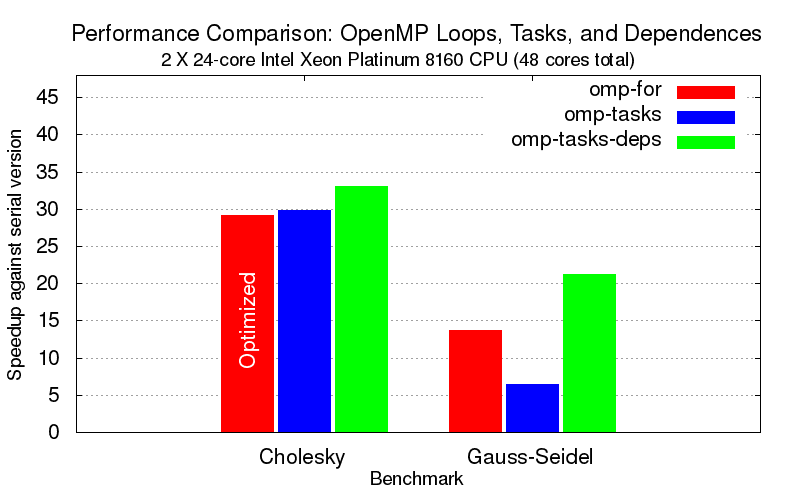
\includegraphics[width=0.45\textwidth]{pics/task-perf-results.png}
\caption{A performance evaluation of task depedendences.}
\label{fig:dep-speedup}
\end{figure}

%% STEPHEN: Discuss task group (example needed or not?)

Recall that all child tasks of the current task must compete at a \texttt{taskwait} construct.  The \texttt{taskgroup} construct allows the current task to wait on only subset of its child tasks, while other child tasks may continue executing beyond the synchronization point.  Additionally, the current task waits on all descendant tasks of the child tasks in the task group, a behavior that may be termed deep synchronization.  Because child tasks of the current task can be excluded from a task group, those tasks could perform long-running background activities that proceed alongside successive computational kernels.


%% STEPHEN: Mention task priorities briefly?

% Michael: the subsubsection is just for my orientation and can be removed.
%\subsubsection{Taskloop}
\label{sec:Taskloop}

The task-based loop, or \emph{taskloop}, is an OpenMP~4.0 extension that enables composition of the tasking model with loop-based parallelism.
Since OpenMP~3.0, the programmer could manually decompose a loop into chunks and assign each chunk to an OpenMP task, but this code transformation was cumbersome and error-prone.
The \code{taskloop} construct automatically transforms a loop into a parallel loop executed using OpenMP tasks.

\begin{figure}
\begin{minted}{c}
void sapxy_tasks(float* a, float* b,
                 float s, size_t n) {
#pragma omp taskloop simd \
            num_tasks(NTASKS) \
            shared(a,b) firstprivate(s)
  for (size_t i = 0; i < n; i++) {
    a[i] = a[i] * b[i] * s;
  }
}
\end{minted}
\caption{Example for using the \code{taskloop} construct.\label{fig:TaskloopExample}}
\end{figure}

Figure~\ref{fig:TaskloopExample} shows the parallelization of a \emph{saxpy} operation using the \code{taskloop} construct.
The \code{num\_tasks} clause specifies the number of OpenMP tasks to create for the sapxy loop.
Alternatively, programmers can use the \code{grainsize} clause to specify the minimum number of loop iterations per task.
The \code{taskloop} construct is also available as a combined construct to use SIMD instructions within the generated tasks.
